\newpage
\subsection{Formalization}

\subsubsection{P.Kocher's DPA mono-bit}
Hereafter is presented the original Differential Power Analysis, also called mono-bit DPA ,
which was published on P.Kocher, J.Jaffe $\&$ B.June, \lokiquote{crypto-1999-kocher}. 
This attack is called mono-bit because the $ f $ function only returns a single bit,
with such a statistical model there is no  need of power model
\textit{i.e.}: 
\begin{center}
$ \;\; f \longrightarrow  \{0,\;1\}$ \\

\vspace{1mm}
$\mathcal{H}=\mathcal{V}$
\end{center}

The principle of this statistical test is to separate traces in two classes or packet
the trace that have been collected from oscilloscope, and then to compute the means of each class.
The way used to separate those trace in two class, noted $G_0$ and  $G_1$, 
lies in the value returned by the function $f$:
\begin{center}
$G_{0,k} := \{\mathcal{C}_i  \| f(M_i,K_k)=0 \} $\\
$G_{1,k} := \{\mathcal{C}_i  \| f(M_i,K_k)=1 \} $
\end{center}
Then is computed the \textit{signal of decision the the sub key $ K_k $}:
\begin{center}
$ \Delta_{K_j}  := \overline{G_{0,k}}-  \overline{G_{1,k}}$
\end{center}

If the hypothesis made is not the good one then the distribution between the two group $G_0$ and $G_1$ are
random and after subtraction the curve of decision  is narrow to zero.
If this hypothesis is good then appears a pic at the moment when the target bit is manipulated, so,
the aim of the attacker is to find the curve with the biggest peak. 
\hspace{3mm}\\

\textbf{advantage:} Robust ans simple

\textbf{inconvenient:} false pike might occurs!\\ 
To avoid this several hypothesis have to be verified:
\begin{itemize}
	\item	the result $ f $ function must be uniformly distributed : 
$\forall k\; \mathbb{P}(f(M_j, K_k)=1) = \frac{1}{2}$
	\item The selection function must have all its output bits independent
	\item The power model have to be relevant 
\end{itemize}

\subsubsection{T-S.Messerge's DPA multi-bit}
Is presented now, an improvement of the previous statistical tools,
and called All-or-Nothing multi-bit DPA, introduced by T-S.Messerges \lokiquote{phd-Messerges-2000}. 
The main idea of this attack is to increase the distance between means with a $f$ function
returning $m$ bits instead of only one.  
\begin{center}
$ \;\; f \longrightarrow  \{0,\;1\}^m$ \\
\end{center}

To achieve this objective curves will be partitioned in three class, here are the two class
that will be used for the computation of the signal of decision:
\begin{center}
$G_{0,k} := \{  \mathcal{C}_i  \| f(M_i,K_k) = \overbrace{0\hdots0}^{m \; bits} \}$\\
$G_{1,k} := \{  \mathcal{C}_i  \| f(M_i,K_k) = \overbrace{1\hdots1}^{m \; bits} \}$\\
\end{center}
And:
\begin{center}
$G_{01,k} = \{  \mathcal{C}_i   \| \mathcal{C}_i    \notin \{ G_{0,k} \cup G_{1,k} \} \}$
\end{center}
The attacker can compute the curve of the distance between the means of each class:
\begin{center}
$ \Delta_{K_j}  := \overline{G_{0,k}}-  \overline{G_{1,k}}$
\end{center}
\textbf{advantage:}

With this method the goods pike will be $m$ times much higher than with mono bit DPA\\
\textbf{inconvenient:}

All curves of $G_{01,k} $ are lost for this attack, which clearly represent
most of them.

In order that multi-bit DPA to be still effective a compromise in the definition
of the partition have to be found, nowadays the most accepted one is: 
\begin{center}
$G_{0,k} := \{  \mathcal{C}_i  \|   \omega_{\mathcal{H}}( f(M_i,K_k) ) < m/2 \}$\\
$G_{1,k} := \{  \mathcal{C}_i  \|   \omega_{\mathcal{H}}( f(M_i,K_k) ) > m/2 \}$\\
\end{center}

\textbf{advantage:} far much relevant than All-or-nothing DPA.\\
\textbf{inconvenient:} If $m$ is odd, some curve won't be used.



\subsubsection{Correlation Power Analysis}
 The main problem with the multi-bit attack previously presented is that all the
curve are not always used when  $m$ is odd which append all the time because all kind of
architecture have an odd number of bits. This point have encourage researchers to find another 
method which would not use a partition of the curves in different classes.

Few years after the publication of  T.Messerges \cite{phd-Messerges-2000} \lokiquote{ches-2004-brier}
published a new method transforming the problem of an attack changing
the problem of detection of a difference of means for a problem of detection 
of a correlation between a set of measures and  a power consumption model.


In DPA attacks, the correlation coefficient is used to determine the linear relationship between
the $i^{th}$ column of $\mathcal{H}$ and the $j^{th}$ column of $\mathcal{T}$ for $i \in\{ 1, \ldots,K \}$
and $j \in\{ 1, \ldots,T \}$. This results in a matrix $\mathcal{R}$ of estimated correlation coefficients.
We estimate each value $r_{i,j}$ based on the D elements of the columns $h_{i}$ and $t_{j}$. So we can
rewrite with the same notation the following formula :
\begin{center}
$r_{i,j} = \frac{\sum_{d=1}^{D}(h_{d,i}-\bar{h_{i}}) . (t_{d,j}-\bar{t_{j}})}{\sqrt{\sum_{d=1}^{D
}(h_{d,i}-\bar{h_{i}})^2} . \sqrt{\sum_{d=1}^{D}(t_{d,j}-\bar{t_{j}})^2}}$
\end{center}


\textbf{advantage:} All the curve are systematically used. 





\subsubsection{Partitioning Power Analysis}

In 2006 a group of researcher composed by T-H.Le, J.Cl\'edi\`ere, C.Canovas,
 B.Robisson, C.S\'ervi\`ere and J-L \lokiquote{ches-2006-lee} presented a new method that 
was generalizing all DPA attacks in the right lineage of \cite{crypto-1999-kocher}.
In order to generalize the multi-bit DPA method, they purpose 
this method defining a large number of packets. 
The concept of multi-partitioning has been suggested by M.L-Akkar and Al, but
these authors did not formalize the concept.

For this method the hypothesis about power consumption have to be done,
so we will begin to explain this attack from the $H$ matrix that has been introduced previously.
The goal, when attacking a DES algorithm, is still to find a part of a round key associated to 
a fixed S-Box.\\
This method can be explain by the following steps :

\begin{itemize}
\item Define packets :
our selection function $f$ is returning $m$ bits, in this case we will defined $m+1$
packets defined with the previous notation :
\begin{center}$\forall \mbox{ }0 \leq j \leq m$: $G_{j,k} := \{\mathcal{C}_i,i=1..N
\|\omega_{\mathcal{H}}(f(M_i,K_k))=j \}$\\
\end{center}
\item Created average : to each packets will be associated the average of the curve 
belonging to it, that will be noted  $\overline{G_{j,k}}$.
\item Computation of the decision signal :
\begin{center}
$ \Delta_{K_j}  := \sum\limits_{j=0}^{m} \; a_{j,k}\;\; \overline{G_{j,k}}$
\end{center}
where $(a_{j,k})_{0 \leq j \leq m }$ are weight that will strongly impacts the performance
of this attack. Those weight can be dependent or not of the key assumption, in our case we have
$ a_{j,k} =  a_j $.
\end{itemize}
 Briefly, the attack works similarly as the DPA,
 the exception is after the step 5 of our DPA description. Indeed, 
we put the traces in $m$ packets, and then we calculate $ \Delta_{K_j}$.
As usually with such a signal decision the curve on which is maximum of this value will 
possibly indicate the correct hypothetical key. 
It's done for one S-box, so we have to do the same with all of them.

\textbf{\textit{Advantages :}}\\
Less curves are necessary to recover a key.\\
As the partition is more precise, the results are much more a{ches-2006-lee}\\
Strong reduction of the false and secondary peaks. The  next figure illustrate it.

\begin{center}
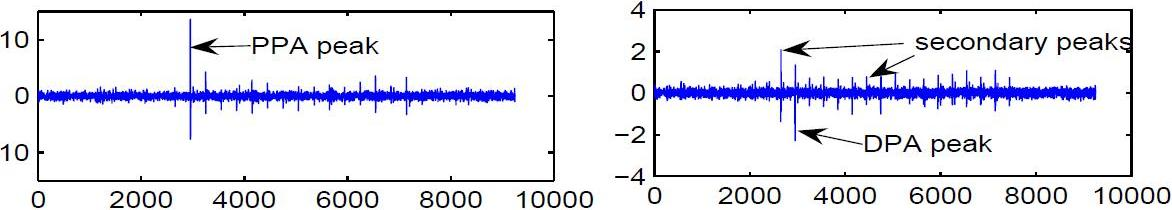
\includegraphics[width=120mm,height=22mm]{images/illustrationPPA.jpg}\\
\textit{Figure 24. Comparison between PPA and DPA for a good key hypothesis}
\end{center}

\textbf{inconvenient:}\\
In the case of $m = 2$, all curve of $G_{2} $ will not be used for the computation of $ \Delta_{K_j} $.


\subsubsection{PPA generalize all previous DPA attacks}

\textbf{1)} For specific values of the weight we are in fact defining well known attacks :\\
$\bullet$ if the values are : $a_0=-1$ and $a_4=1$ and other set to 0 it's the P.Kocker mono-bit DPA.\\
$\bullet$ if the values are :
\begin{center}
 $ a_j =\left\{ \begin{array}{ll}  -1$ if $0 \leq j < m/2 \\\;\;1$ if $m/2 \leq j \leq d\end{array} \right.$
\end{center} 
it's the P.Kocher mono-bit DPA.\\
it's the  all T.Messerges multi-bit DPA and OAN-DPA.\\
\textbf{2)} The reader can also read the demonstration which explain that the CPA
is also a particular case of PPA for some specific values of $a_j$.\\
\textbf{3)} Optimal values for weights are $(a_j)_{0 \leq j \leq m  } = \{-1,-2,0,2,1\}$, 
this set of weights is maximizing the Signal Noise Ratio for the linear model of power consumption. 
See \lokiquote{asiacs-2008-Lee}.

\subsubsection{Maximum of probability}
This method was invented by R.Bevan and E.Knudsen [1]. This method takes into account
 what appends when the amount of current to pass a bit from 0 to 1 is different from that needed to pass a
  bit from 1 to 0. 
With the model of consumption we have :
\begin{center}
$\mathcal{C}_{i}=\sum_{k=1}^{p}\lambda_{ki} \theta_{k} + w_{i}$,
\end{center}
which $\theta_{k}$ is the parameters of the consumption model and p the number of parameters.\\
For $N$ different consumption measures, we have the matrix relation :
\begin{center}
\begin{displaymath}
\mathcal{C}=
\left(\begin{array}{ccc}
\mathcal{C}_{1} \\
\vdots \\
\mathcal{C}_{N} \\
\end{array}\right)
=
\left( \begin{array}{cccc}
\lambda_{1,1} & \lambda_{2,1} & \ldots & \lambda_{p,1} \\
\vdots        & \vdots        &        & \vdots \\
\lambda_{1,N} & \lambda_{2,N} & \ldots & \lambda_{p,N}\\
\end{array} \right) 
\left( \begin{array}{ccc}
\theta_{1} \\
\vdots \\
\theta_{N} \\
\end{array} \right)
+
\left( \begin{array}{ccc}
w_{1} \\
\vdots \\
w_{N} \\
\end{array} \right)
\end{displaymath}
\end{center}

with this notation the attacker will keep the key which maximize the following relation :
\begin{center}
$L_{K_{j}}=\frac{N}{2} ( ln({}^t \! \mathcal{C} . \mathcal{C} - \frac{1}{N}(\sum_{i=1}^{N}\mathcal{C}_{i})^2)
- ln({}^t \! \mathcal{C} . \mathcal{C} -ln({}^t \! \mathcal{C} . \lambda_{K_{j}}.( {}^t \! \lambda_{K_{j}}.
\lambda_{K_{j}})^{-1} . {}^t \! \lambda_{K_{j}}.\mathcal{C}))$
\end{center}

\newpage
\subsection{Compare those methods}
Reference
The two references could be :
\begin{itemize}
	\item In 2004 Regis Bevan PhD in \lokiquote{phd-Bevan-2004}: are compared mono-bit, 'All or Nothing multi bit DPA', multi bit DPA and CPA.
	\item In 2011 Julien Doget's article \lokiquote{jce-2011-doget} : much more comparison, ultimately clear notations.
\end{itemize} 

Hereafter picture beeing taken from the excellent article of Julien Doget, 
a comparison in term of efficiency between many statistical methods. 
Note that mono bit DPA return bit of key whereas the other return 6.

\begin{center}
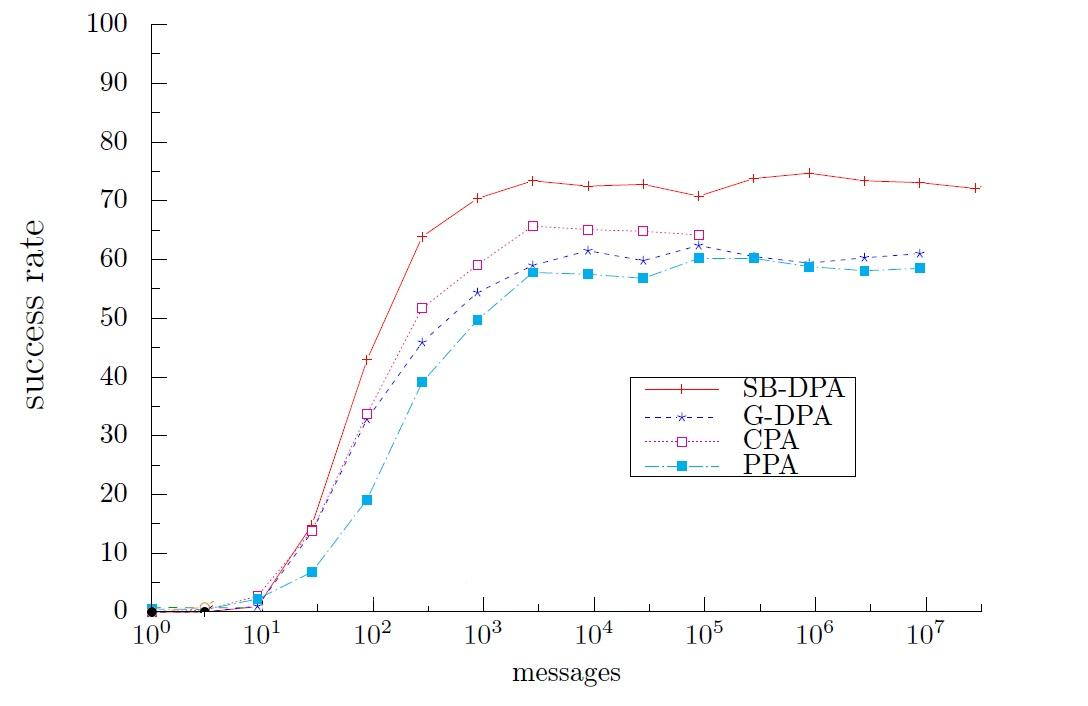
\includegraphics[width=140mm,height=95mm]{images/compare.jpg}\\
\end{center}
